\chapter{Sentiment Analysis}
	????????????

	\section{Scelta delle top three category}
		Il nostro primo obiettivo è quello di studiare l'intrattenimento, in particolare quali siano i prodotti più recensiti all'interno delle nostre quattro categorie. Come primo passo abbiamo  quindi scelto di effettuare lo studio su un numero limitato di prodotti, riducendoli a duecento, e di analizzare la loro distribuzione. I risultati ottenuti sono presentati nella Figura \ref{fig:pie_category}
		
		\begin{figure} [h]
			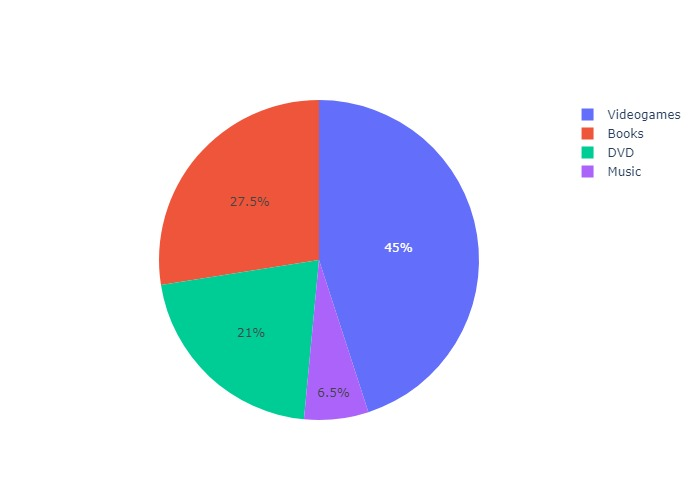
\includegraphics[width=\textwidth]{Figure/pie_category}
			\caption{Distribuzione delle recensioni per ogni categoria.}
			\label{fig:pie_category}
		\end{figure}
	
		Dalla figura è possibile notare che, in percentuale, i prodotti più recensiti appartengono alla categoria dei videogiochi (\verb|45%|), seguiti dai libri (\verb|27.5%|), dai dvd (\verb|21%|) e dalla musica (\verb|6.5%|). Quest'ultima categoria è davvero esigua perché delle analisi diano risultati consistenti e si possano ricavare informazioni utili; inoltre poiché lo studio su cui abbiamo posto l'attenzione riguardava i più popolari, non aveva senso esaminare dei prodotti quasi privi di recensioni. Da questa considerazione è derivata la scelta di escludere \verb|music| e procedere ad analizzare l'intrattenimento solo sulle tre migliori categorie, quindi \verb|videogames|, \verb|books| e \verb|dvd|. Arrivati a questo punto il nostro studio è stato diviso in due diversi passaggi; nel primo siamo andati a cercare i prodotti meglio recensiti e quelli con più recensioni negative; mentre nel secondo passaggio abbiamo ricostruito quali fossero le parole più usate all'interno dei due diversi insiemi di recensioni. 
		
		\subsection{Primo passaggio: distribuzione del sentiment}
			Come già accennato, per poter valutare la polarità di una recensione è necessario calcolare il \textit{sentiment}. Abbiamo visto che questo calcolo può essere eseguito secondo diverse metodologie, tuttavia il nostro \textit{dataset} relativo ai prodotti, presentava al suo interno un campo che ben si prestava a questo tipo di analisi. L'attributo in questione è quello delle stelle. \textit{Amazon} infatti per ogni recensione riferita a un determinato prodotto associa una valutazione in stelle da \verb|0| a \verb|5|. Questo ha permesso di effettuare un conteggio per ogni prodotto di tutte le sue recensioni, dividendole in positive negative e neutre, secondo lo schema di seguito.
			
			\begin{itemize}
				\item \textbf{positive:} la recensione aveva un punteggio di maggiore di tre stelle.
				\item \textbf{neuter:} la recensione aveva un punteggio uguale a tre stelle.
				\item \textbf{negative:} la recensione aveva un punteggio minore di tre stelle.
			\end{itemize}
			
			Procedendo secondo queste modalità, preso per esempio il prodotto "Zelda", con \verb|200| recensioni, si calcolano quante di queste sono risultate positive negative oppure neutre e un possibile risultato potrebbe essere costituito da \verb|100| recensioni positive, \verb|70| negative e \verb|30| neutre. \\		
			Ottenuto questo elenco abbiamo calcolato la distribuzione probabilistica associata alle tre diverse polarità. In particolare per ognuna associata a uno specifico prodotto, abbiamo effettuato un rapporto tra il conteggio delle recensioni positive e negative, escludendo le neutre (dato non rilevante per la nostra analisi) e il numero di recensioni totali. 
			
			La distribuzione probabilistica della polarità ottenuta è stata quindi combinata al sottoinsieme dei prodotti più recensiti/più popolari e il risultato di questo \textit{match} è stata l'identificazione per ogni categoria dei prodotti più popolari suddivisi in due elenchi. Il primo contenente i prodotti valutati più negativamente e nel secondo quelli valutati più positivamente. \\
			I risultati ottenuti sono visibili nelle Figure \ref{fig:top_pos_book_table} \ref{fig:top_neg_book_table}, \ref{fig:top_pos_film_table}, \ref{fig:top_neg_film_table}, \ref{fig:top_pos_videogames_table}, \ref{fig:top_neg_videogames_table}.
			
			\begin{figure} [h]
				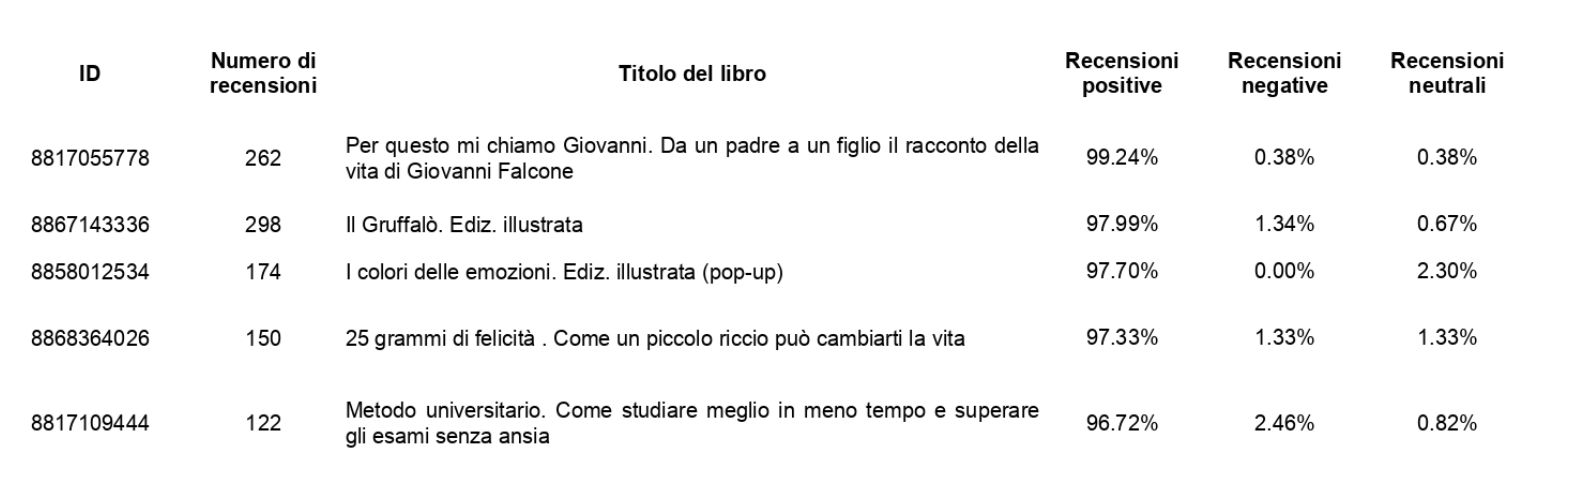
\includegraphics[width=\textwidth]{Figure/top_pos_book_table}
				\caption{Primi cinque libri con più recensioni positive}
				\label{fig:top_pos_book_table}
			\end{figure}
			
			\begin{figure} [h]
				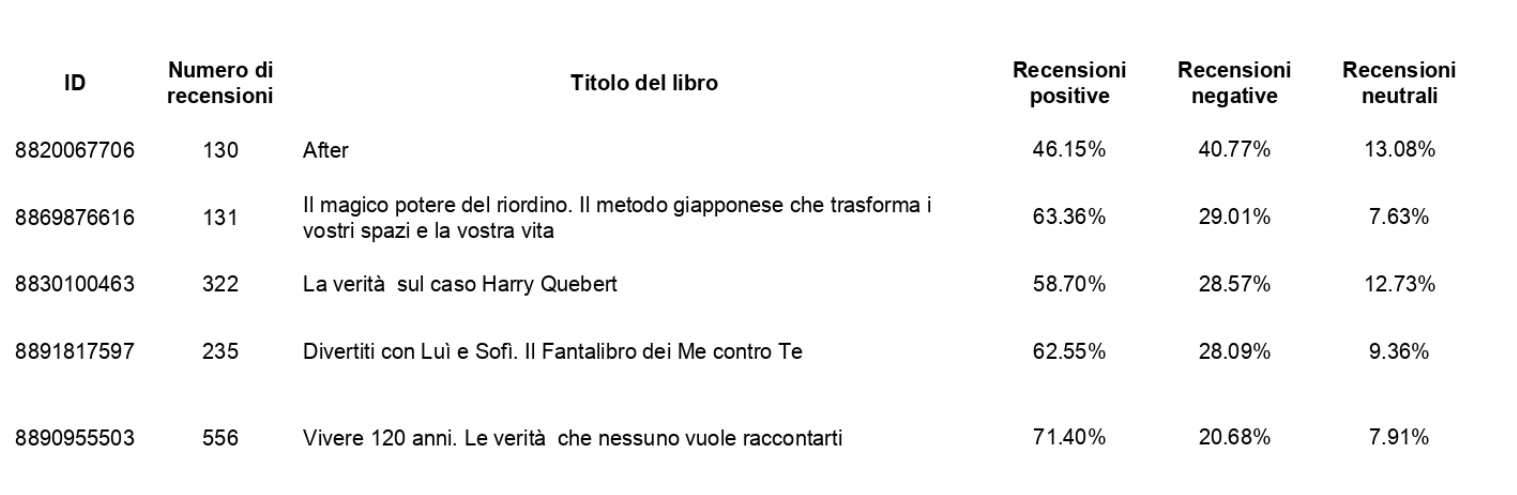
\includegraphics[width=\textwidth]{Figure/top_neg_book_table}
				\caption{Primi cinque libri con più recensioni negative}
				\label{fig:top_neg_book_table}
			\end{figure}
		
			\begin{figure} [h]
				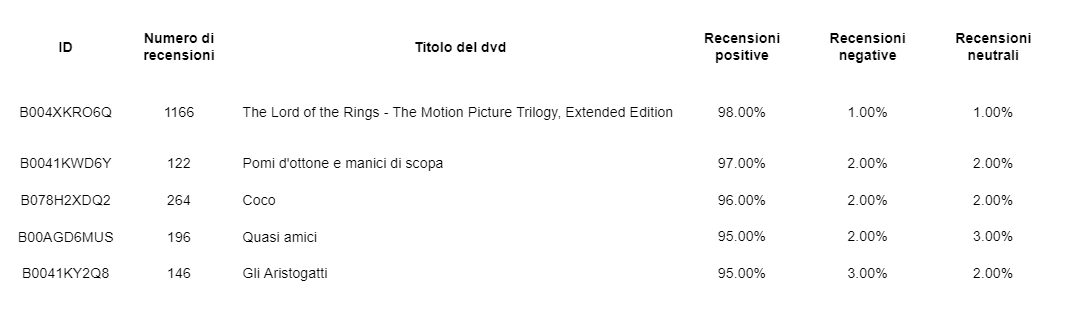
\includegraphics[width=\textwidth]{Figure/top_pos_film_table}
				\caption{Primi cinque dvd con più recensioni positive}
				\label{fig:top_pos_film_table}
			\end{figure}
		
			\begin{figure} [h]
				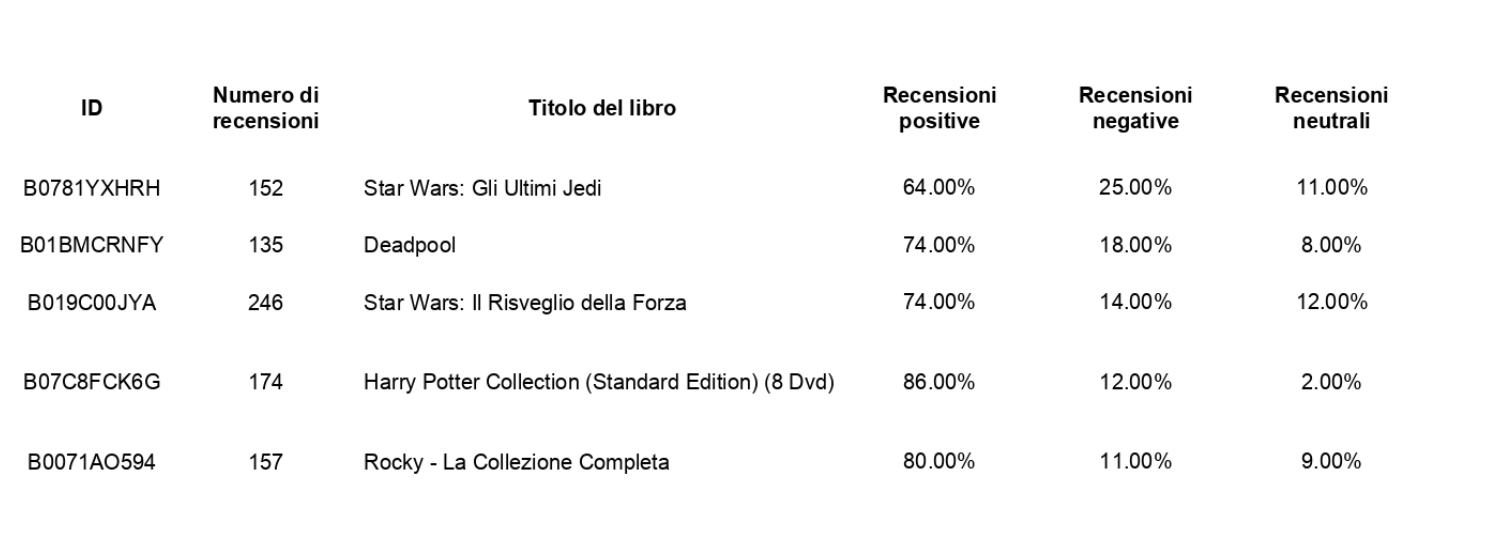
\includegraphics[width=\textwidth]{Figure/top_neg_film_table}
				\caption{Primi cinque dvd con più recensioni negative}
				\label{fig:top_neg_film_table}
			\end{figure}
		
			\begin{figure} [h]
				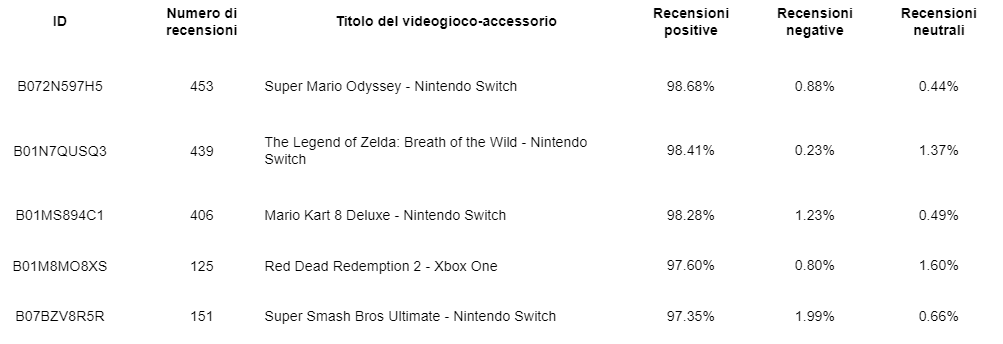
\includegraphics[width=\textwidth]{Figure/top_pos_videogames_table}
				\caption{Primi cinque videogiochi con più recensioni positive}
				\label{fig:top_pos_videogames_table}
			\end{figure}
		
			\begin{figure} [h]
				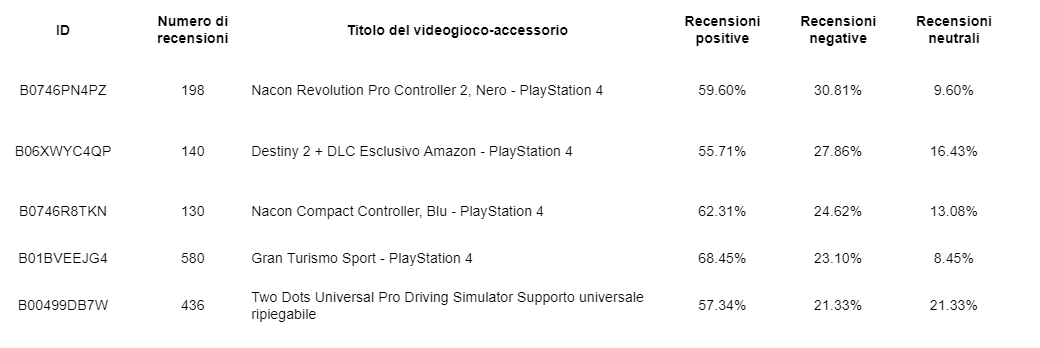
\includegraphics[width=\textwidth]{Figure/top_neg_videogames_table}
				\caption{Primi cinque videogiochi con più recensioni negative}
				\label{fig:top_neg_videogames_table}
			\end{figure}
		
\pagebreak	
		\subsection{Secondo passaggio: analisi delle parole più usate}
			
		Per poter eseguire delle analisi consistenti sono indispensabili una serie di operazioni atti a uniformare il \textit{dataset}. Con il termine "uniformare" intendiamo riscrivere i dati seguendo delle specifiche regole comuni. Nel seguito ogni procedura verrà descritta nel dettaglio.
		
		
		